\documentclass[12pt]{article} 
\usepackage[margin=2cm]{geometry} 
\usepackage{psfrag} 
\usepackage{graphicx} 
\usepackage{epstopdf} 
\usepackage{longtable,booktabs} 
\usepackage{amsmath,amsfonts} 
\usepackage{breqn} 
\usepackage{float,morefloats,caption} 
\begin{document} 
% 23-Jan-2024 16:35:14, created by McMCDiagnostics.m 
 
\begin{center}
\begin{longtable}{lcc} 
\caption{MCMC Inefficiency factors per block}\\
 \label{Table:MCMC_inefficiency_factors}\\
\toprule 
$Parameter          $	 & 	 $     Block~1$	 & 	 $     Block~2$\\
\midrule \endfirsthead 
\caption{(continued)}\\
 \toprule \\ 
$Parameter          $	 & 	 $     Block~1$	 & 	 $     Block~2$\\
\midrule \endhead 
\midrule \multicolumn{3}{r}{(Continued on next page)} \\ \bottomrule \endfoot 
\bottomrule \endlastfoot 
$ \sigma_{{e_ZI}}   $	 & 	     488.250	 & 	     464.099 \\ 
$ \sigma_{{e_Z}}    $	 & 	     613.961	 & 	     580.273 \\ 
$ \sigma_{{e_N}}    $	 & 	     548.772	 & 	     550.104 \\ 
$ \sigma_{{e_D}}    $	 & 	     290.988	 & 	     221.325 \\ 
$ {\rho_Z}          $	 & 	      92.013	 & 	      80.247 \\ 
$ {\rho_ZI}         $	 & 	     732.176	 & 	     708.002 \\ 
$ {\rho_N}          $	 & 	     512.506	 & 	     472.244 \\ 
$ {\rho_D}          $	 & 	     447.667	 & 	     435.102 \\ 
\end{longtable}
 \end{center}
% End of TeX file.
 
\include{BRS/latex/BRS_latex_definitions} 
\begin{center}
\begin{longtable}{ccc}
\caption{Parameter Values}\\%
\toprule%
\multicolumn{1}{c}{\textbf{Parameter}} &
\multicolumn{1}{c}{\textbf{Value}} &
 \multicolumn{1}{c}{\textbf{Description}}\\%
\midrule%
\endfirsthead
\multicolumn{3}{c}{{\tablename} \thetable{} -- Continued}\\%
\midrule%
\multicolumn{1}{c}{\textbf{Parameter}} &
\multicolumn{1}{c}{\textbf{Value}} &
  \multicolumn{1}{c}{\textbf{Description}}\\%
\midrule%
\endhead
${\gamma}$ 	 & 	 1.000 	 & 	 Risk aversion\\
${r_ann}$ 	 & 	 0.040 	 & 	 Annual interest rate\\
${\overline{g}}$ 	 & 	 0.000 	 & 	 Quarterly growth rate\\
$(\nu)$ 	 & 	 0.720 	 & 	 Frisch elasticity\\
$(I_Y)$ 	 & 	 0.200 	 & 	 Investment-output ratio\\
$(K_Y)$ 	 & 	 11.000 	 & 	 Capital-output ratio (quarterly)\\
$(labor share)$ 	 & 	 0.670 	 & 	 Labor share\\
$(\phi)$ 	 & 	 0.320 	 & 	 Shopping matching function elasticity\\
$(\eta)$ 	 & 	 0.200 	 & 	 Shopping disutility\\
$(\Psi)$ 	 & 	 0.810 	 & 	 Matching utilization\\
${\rho_Z}$ 	 & 	 0.999 	 & 	 persistence TFP shock\\
${\rho_ZI}$ 	 & 	 0.733 	 & 	 persistence I-specific shock\\
${\rho_N}$ 	 & 	 0.944 	 & 	 persistence labor supply shock\\
${\rho_D}$ 	 & 	 0.825 	 & 	 persistence shopping effort shock\\
$p\_I\_ss$ 	 & 	 1.000 	 & 	 p\_I\_ss\\
$N\_ss$ 	 & 	 0.300 	 & 	 N\_ss\\
\bottomrule%
\end{longtable}
\end{center}
 
\include{BRS/latex/BRS_priors_table} 
\begin{dmath*}
r = \left(1+{{r_ann}}\right)^{0.25}-1.0
\end{dmath*}
\begin{dmath*}
I\_K = \frac{{{I_Y}}}{{{K_Y}}}
\end{dmath*}
\begin{dmath*}
delta = 1+\frac{{{I_Y}}}{{{K_Y}}}-\exp\left({{\overline{g}}}\right)
\end{dmath*}
\begin{dmath*}
alpha\_K = {{K_Y}}\, \left(\left(1+{{r_ann}}\right)^{0.25}-1.0+1+\frac{{{I_Y}}}{{{K_Y}}}-\exp\left({{\overline{g}}}\right)\right)
\end{dmath*}
\begin{dmath*}
beta = \exp\left({{\overline{g}}}\right)^{{{\gamma}}}\, \frac{1}{1+\left(1+{{r_ann}}\right)^{0.25}-1.0}
\end{dmath*}
\begin{dmath*}
sigma\_b = \left(1+{{r_ann}}\right)^{0.25}-1.0+1+\frac{{{I_Y}}}{{{K_Y}}}-\exp\left({{\overline{g}}}\right)
\end{dmath*}
\begin{dmath*}
phi = \frac{\left(1+{{\eta}}\right)\, {{m}}}{1+{{\eta}}\, {{m}}}
\end{dmath*}
\begin{dmath*}
alpha\_N = {(labor share)}\, \left(1-\frac{\left(1+{{\eta}}\right)\, {{m}}}{1+{{\eta}}\, {{m}}}\right)
\end{dmath*}
\begin{dmath*}
D\_ss = \left(\frac{\left(1+{{\eta}}\right)\, {{m}}}{1+{{\eta}}\, {{m}}}\right)^{\frac{{{\eta}}}{1+{{\eta}}}}
\end{dmath*}
\begin{dmath*}
D\_C\_ss = \left(1-{{I_Y}}\right)\, \left(\frac{\left(1+{{\eta}}\right)\, {{m}}}{1+{{\eta}}\, {{m}}}\right)^{\frac{{{\eta}}}{1+{{\eta}}}}
\end{dmath*}
\begin{dmath*}
D\_I\_ss = {{I_Y}}\, \left(\frac{\left(1+{{\eta}}\right)\, {{m}}}{1+{{\eta}}\, {{m}}}\right)^{\frac{{{\eta}}}{1+{{\eta}}}}
\end{dmath*}
\begin{dmath*}
A\_C = \frac{{{\Psi}}}{\left(\left(1-{{I_Y}}\right)\, \left(\frac{\left(1+{{\eta}}\right)\, {{m}}}{1+{{\eta}}\, {{m}}}\right)^{\frac{{{\eta}}}{1+{{\eta}}}}\right)^{\frac{\left(1+{{\eta}}\right)\, {{m}}}{1+{{\eta}}\, {{m}}}}}
\end{dmath*}
\begin{dmath*}
A\_I = \frac{{{\Psi}}}{\left({{I_Y}}\, \left(\frac{\left(1+{{\eta}}\right)\, {{m}}}{1+{{\eta}}\, {{m}}}\right)^{\frac{{{\eta}}}{1+{{\eta}}}}\right)^{\frac{\left(1+{{\eta}}\right)\, {{m}}}{1+{{\eta}}\, {{m}}}}}
\end{dmath*}
\begin{dmath*}
I\_ss = {{I_Y}}
\end{dmath*}
\begin{dmath*}
C\_ss = 1-{{I_Y}}
\end{dmath*}
\begin{dmath*}
K\_ss = {{K_Y}}\, \exp\left({{\overline{g}}}\right)
\end{dmath*}
\begin{dmath*}
K\_I\_ss = {{I_Y}}\, {{K_Y}}\, \exp\left({{\overline{g}}}\right)
\end{dmath*}
\begin{dmath*}
K\_C\_ss = \left(1-{{I_Y}}\right)\, {{K_Y}}\, \exp\left({{\overline{g}}}\right)
\end{dmath*}
\begin{dmath*}
N\_I\_ss = {{I_Y}}\, {N\_ss}
\end{dmath*}
\begin{dmath*}
N\_C\_ss = \left(1-{{I_Y}}\right)\, {N\_ss}
\end{dmath*}
\begin{dmath*}
omega = 1-{{I_Y}}
\end{dmath*}
\begin{dmath*}
W\_ss = \frac{{{I_Y}}\, {(labor share)}\, \left(1-\frac{\left(1+{{\eta}}\right)\, {{m}}}{1+{{\eta}}\, {{m}}}\right)\, \frac{{p\_I\_ss}}{1-\frac{\left(1+{{\eta}}\right)\, {{m}}}{1+{{\eta}}\, {{m}}}}}{{{I_Y}}\, {N\_ss}}
\end{dmath*}
\begin{dmath*}
Z\_C\_ss = \frac{1-{{I_Y}}}{{{\Psi}}\, \exp\left({{\overline{g}}}\right)^{\left(-\left({{K_Y}}\, \left(\left(1+{{r_ann}}\right)^{0.25}-1.0+1+\frac{{{I_Y}}}{{{K_Y}}}-\exp\left({{\overline{g}}}\right)\right)\right)\right)}\, \left(\left(1-{{I_Y}}\right)\, {{K_Y}}\, \exp\left({{\overline{g}}}\right)\right)^{{{K_Y}}\, \left(\left(1+{{r_ann}}\right)^{0.25}-1.0+1+\frac{{{I_Y}}}{{{K_Y}}}-\exp\left({{\overline{g}}}\right)\right)}\, \left(\left(1-{{I_Y}}\right)\, {N\_ss}\right)^{{(labor share)}\, \left(1-\frac{\left(1+{{\eta}}\right)\, {{m}}}{1+{{\eta}}\, {{m}}}\right)}}
\end{dmath*}
\begin{dmath*}
Z\_I\_ss = \frac{{{I_Y}}}{{{\Psi}}\, \exp\left({{\overline{g}}}\right)^{\left(-\left({{K_Y}}\, \left(\left(1+{{r_ann}}\right)^{0.25}-1.0+1+\frac{{{I_Y}}}{{{K_Y}}}-\exp\left({{\overline{g}}}\right)\right)\right)\right)}\, \left({{I_Y}}\, {{K_Y}}\, \exp\left({{\overline{g}}}\right)\right)^{{{K_Y}}\, \left(\left(1+{{r_ann}}\right)^{0.25}-1.0+1+\frac{{{I_Y}}}{{{K_Y}}}-\exp\left({{\overline{g}}}\right)\right)}\, \left({{I_Y}}\, {N\_ss}\right)^{{(labor share)}\, \left(1-\frac{\left(1+{{\eta}}\right)\, {{m}}}{1+{{\eta}}\, {{m}}}\right)}}
\end{dmath*}
\begin{dmath*}
theta\_N\_ss = \frac{\left(1-\frac{\left(1+{{\eta}}\right)\, {{m}}}{1+{{\eta}}\, {{m}}}\right)\, \frac{{{I_Y}}\, {(labor share)}\, \left(1-\frac{\left(1+{{\eta}}\right)\, {{m}}}{1+{{\eta}}\, {{m}}}\right)\, \frac{{p\_I\_ss}}{1-\frac{\left(1+{{\eta}}\right)\, {{m}}}{1+{{\eta}}\, {{m}}}}}{{{I_Y}}\, {N\_ss}}}{{{N}}_{t}^{\frac{1}{{\nu}}}}
\end{dmath*}
% Equation 1
\begin{dmath}
{{N}}_{t}=\left({{N_C}}_{t}^{1+{{\theta}}}\, \left(1-{{I_Y}}\right)^{\left(-{{\theta}}\right)}+{{N_I}}_{t}^{1+{{\theta}}}\, \left(1-\left(1-{{I_Y}}\right)\right)^{\left(-{{\theta}}\right)}\right)^{\frac{1}{1+{{\theta}}}}
\end{dmath}
% Equation 2
\begin{dmath}
{{N}}_{t}^{\frac{1}{{\nu}}}\, \exp\left({{\theta_N}}_{t}\right)\, \frac{\left(1-\frac{\left(1+{{\eta}}\right)\, {{m}}}{1+{{\eta}}\, {{m}}}\right)\, \frac{{{I_Y}}\, {(labor share)}\, \left(1-\frac{\left(1+{{\eta}}\right)\, {{m}}}{1+{{\eta}}\, {{m}}}\right)\, \frac{{p\_I\_ss}}{1-\frac{\left(1+{{\eta}}\right)\, {{m}}}{1+{{\eta}}\, {{m}}}}}{{{I_Y}}\, {N\_ss}}}{{{N}}_{t}^{\frac{1}{{\nu}}}}={{W}}_{t}\, \exp\left({{\theta_C}}_{t}\right)\, \left(1-\frac{\left(1+{{\eta}}\right)\, {{m}}}{1+{{\eta}}\, {{m}}}\right)
\end{dmath}
% Equation 3
\begin{dmath}
\exp\left({{\theta_D}}_{t}\right)\, {{D}}_{t}^{\frac{1}{{{\eta}}}}=\frac{{{C}}_{t}\, \frac{\left(1+{{\eta}}\right)\, {{m}}}{1+{{\eta}}\, {{m}}}\, \exp\left({{\theta_C}}_{t}\right)}{{{D}}_{t}}
\end{dmath}
% Equation 4
\begin{dmath}
\exp\left({{\theta_D}}_{t}\right)\, {{D}}_{t}^{\frac{1}{{{\eta}}}}=\frac{{{I}}_{t}\, {{p_I}}_{t}\, \frac{\left(1+{{\eta}}\right)\, {{m}}}{1+{{\eta}}\, {{m}}}\, \exp\left({{\theta_C}}_{t}\right)}{{{D}}_{t}}
\end{dmath}
% Equation 5
\begin{dmath}
{{\Gamma}}_{t}=\exp\left({{\theta_C}}_{t}\right)\, {{C}}_{t}-\frac{\exp\left({{\theta_D}}_{t}\right)\, {{D}}_{t}^{1+\frac{1}{{{\eta}}}}}{1+\frac{1}{{{\eta}}}}-\frac{{{N}}_{t}^{1+\frac{1}{{\nu}}}\, \exp\left({{\theta_N}}_{t}\right)\, \frac{\left(1-\frac{\left(1+{{\eta}}\right)\, {{m}}}{1+{{\eta}}\, {{m}}}\right)\, \frac{{{I_Y}}\, {(labor share)}\, \left(1-\frac{\left(1+{{\eta}}\right)\, {{m}}}{1+{{\eta}}\, {{m}}}\right)\, \frac{{p\_I\_ss}}{1-\frac{\left(1+{{\eta}}\right)\, {{m}}}{1+{{\eta}}\, {{m}}}}}{{{I_Y}}\, {N\_ss}}}{{{N}}_{t}^{\frac{1}{{\nu}}}}}{1+\frac{1}{{\nu}}}-{{\zeta}}\, {{ha}}_{t}
\end{dmath}
% Equation 6
\begin{dmath}
{{ha}}_{t}=\exp\left({{\theta_C}}_{t}\right)\, {{C}}_{t-1}-\frac{\exp\left({{\theta_D}}_{t}\right)\, {{D}}_{t-1}^{1+\frac{1}{{{\eta}}}}}{1+\frac{1}{{{\eta}}}}-\frac{{{N}}_{t-1}^{1+\frac{1}{{\nu}}}\, \exp\left({{\theta_N}}_{t}\right)\, \frac{\left(1-\frac{\left(1+{{\eta}}\right)\, {{m}}}{1+{{\eta}}\, {{m}}}\right)\, \frac{{{I_Y}}\, {(labor share)}\, \left(1-\frac{\left(1+{{\eta}}\right)\, {{m}}}{1+{{\eta}}\, {{m}}}\right)\, \frac{{p\_I\_ss}}{1-\frac{\left(1+{{\eta}}\right)\, {{m}}}{1+{{\eta}}\, {{m}}}}}{{{I_Y}}\, {N\_ss}}}{{{N}}_{t}^{\frac{1}{{\nu}}}}}{1+\frac{1}{{\nu}}}
\end{dmath}
% Equation 7
\begin{dmath}
{{Q}}_{t}=\frac{{{p_I}}_{t}}{1-\frac{\left(1+{{\eta}}\right)\, {{m}}}{1+{{\eta}}\, {{m}}}}\, \left(1-{{\Psi_K}}\, \left({{x}}_{t}-\frac{{{I_Y}}}{{{K_Y}}}\right)\right)^{\left(-1\right)}
\end{dmath}
% Equation 8
\begin{dmath}
{{Q}}_{t}=\left({{R_C}}_{t+1}\, {{h_C}}_{t+1}+{{Q}}_{t+1}\, \left(1-{{\delta_C}}_{t+1}+{{x}}_{t+1}\, {{\Psi_K}}\, \left({{x}}_{t+1}-\frac{{{I_Y}}}{{{K_Y}}}\right)-\frac{{{\Psi_K}}}{2}\, \left({{x}}_{t+1}-\frac{{{I_Y}}}{{{K_Y}}}\right)^{2}\right)\right)\, \exp\left({{g}}_{t+1}\right)^{\left(-{{\gamma}}\right)}\, \left(\frac{{{\Gamma}}_{t+1}}{{{\Gamma}}_{t}}\right)^{\left(-{{\gamma}}\right)}\, \frac{\exp\left({{\theta_C}}_{t+1}\right)\, \exp\left({{\overline{g}}}\right)^{{{\gamma}}}\, \frac{1}{1+\left(1+{{r_ann}}\right)^{0.25}-1.0}}{\exp\left({{\theta_C}}_{t}\right)}
\end{dmath}
% Equation 9
\begin{dmath}
{{Q}}_{t}=\left({{R_I}}_{t+1}\, {{h_I}}_{t+1}+{{Q}}_{t+1}\, \left(1-{{\delta_I}}_{t+1}+{{x}}_{t+1}\, {{\Psi_K}}\, \left({{x}}_{t+1}-\frac{{{I_Y}}}{{{K_Y}}}\right)-\frac{{{\Psi_K}}}{2}\, \left({{x}}_{t+1}-\frac{{{I_Y}}}{{{K_Y}}}\right)^{2}\right)\right)\, \exp\left({{g}}_{t+1}\right)^{\left(-{{\gamma}}\right)}\, \left(\frac{{{\Gamma}}_{t+1}}{{{\Gamma}}_{t}}\right)^{\left(-{{\gamma}}\right)}\, \frac{\exp\left({{\theta_C}}_{t+1}\right)\, \exp\left({{\overline{g}}}\right)^{{{\gamma}}}\, \frac{1}{1+\left(1+{{r_ann}}\right)^{0.25}-1.0}}{\exp\left({{\theta_C}}_{t}\right)}
\end{dmath}
% Equation 10
\begin{dmath}
{{x}}_{t}=\frac{{{I}}_{t}}{{{K}}_{t-1}}\, \exp\left({{g}}_{t}\right)
\end{dmath}
% Equation 11
\begin{dmath}
{{Q}}_{t}\, {{\delta_C}}_{t}={{R_C}}_{t}
\end{dmath}
% Equation 12
\begin{dmath}
{{Q}}_{t}\, {{\delta_I}}_{t}={{R_I}}_{t}
\end{dmath}
% Equation 13
\begin{dmath}
{{\delta_C}}_{t}=1+\frac{{{I_Y}}}{{{K_Y}}}-\exp\left({{\overline{g}}}\right)+\left({{h_C}}_{t}-1\right)\, \left(\left(1+{{r_ann}}\right)^{0.25}-1.0+1+\frac{{{I_Y}}}{{{K_Y}}}-\exp\left({{\overline{g}}}\right)\right)+\left({{h_C}}_{t}-1\right)^{2}\, \frac{{{\sigma_a}}\, \left(\left(1+{{r_ann}}\right)^{0.25}-1.0+1+\frac{{{I_Y}}}{{{K_Y}}}-\exp\left({{\overline{g}}}\right)\right)}{2}
\end{dmath}
% Equation 14
\begin{dmath}
{{\delta_I}}_{t}=1+\frac{{{I_Y}}}{{{K_Y}}}-\exp\left({{\overline{g}}}\right)+\left({{h_I}}_{t}-1\right)\, \left(\left(1+{{r_ann}}\right)^{0.25}-1.0+1+\frac{{{I_Y}}}{{{K_Y}}}-\exp\left({{\overline{g}}}\right)\right)+\left({{h_I}}_{t}-1\right)^{2}\, \frac{{{\sigma_a}}\, \left(\left(1+{{r_ann}}\right)^{0.25}-1.0+1+\frac{{{I_Y}}}{{{K_Y}}}-\exp\left({{\overline{g}}}\right)\right)}{2}
\end{dmath}
% Equation 15
\begin{dmath}
{{\delta_C}}_{t}=\left(1+{{r_ann}}\right)^{0.25}-1.0+1+\frac{{{I_Y}}}{{{K_Y}}}-\exp\left({{\overline{g}}}\right)+\left({{h_C}}_{t}-1\right)\, {{\sigma_a}}\, \left(\left(1+{{r_ann}}\right)^{0.25}-1.0+1+\frac{{{I_Y}}}{{{K_Y}}}-\exp\left({{\overline{g}}}\right)\right)
\end{dmath}
% Equation 16
\begin{dmath}
{{\delta_I}}_{t}=\left(1+{{r_ann}}\right)^{0.25}-1.0+1+\frac{{{I_Y}}}{{{K_Y}}}-\exp\left({{\overline{g}}}\right)+\left({{h_I}}_{t}-1\right)\, {{\sigma_a}}\, \left(\left(1+{{r_ann}}\right)^{0.25}-1.0+1+\frac{{{I_Y}}}{{{K_Y}}}-\exp\left({{\overline{g}}}\right)\right)
\end{dmath}
% Equation 17
\begin{dmath}
{{C}}_{t}=\exp\left({{Z_C}}_{t}\right)\, \frac{1-{{I_Y}}}{{{\Psi}}\, \exp\left({{\overline{g}}}\right)^{\left(-\left({{K_Y}}\, \left(\left(1+{{r_ann}}\right)^{0.25}-1.0+1+\frac{{{I_Y}}}{{{K_Y}}}-\exp\left({{\overline{g}}}\right)\right)\right)\right)}\, \left(\left(1-{{I_Y}}\right)\, {{K_Y}}\, \exp\left({{\overline{g}}}\right)\right)^{{{K_Y}}\, \left(\left(1+{{r_ann}}\right)^{0.25}-1.0+1+\frac{{{I_Y}}}{{{K_Y}}}-\exp\left({{\overline{g}}}\right)\right)}\, \left(\left(1-{{I_Y}}\right)\, {N\_ss}\right)^{{(labor share)}\, \left(1-\frac{\left(1+{{\eta}}\right)\, {{m}}}{1+{{\eta}}\, {{m}}}\right)}}\, {{D}}_{t}^{\frac{\left(1+{{\eta}}\right)\, {{m}}}{1+{{\eta}}\, {{m}}}}\, \frac{{{\Psi}}}{\left(\left(1-{{I_Y}}\right)\, \left(\frac{\left(1+{{\eta}}\right)\, {{m}}}{1+{{\eta}}\, {{m}}}\right)^{\frac{{{\eta}}}{1+{{\eta}}}}\right)^{\frac{\left(1+{{\eta}}\right)\, {{m}}}{1+{{\eta}}\, {{m}}}}}\, \exp\left({{g}}_{t}\right)^{\left(-\left({{K_Y}}\, \left(\left(1+{{r_ann}}\right)^{0.25}-1.0+1+\frac{{{I_Y}}}{{{K_Y}}}-\exp\left({{\overline{g}}}\right)\right)\right)\right)}\, \left({{h_C}}_{t}\, {{K_C}}_{t-1}\right)^{{{K_Y}}\, \left(\left(1+{{r_ann}}\right)^{0.25}-1.0+1+\frac{{{I_Y}}}{{{K_Y}}}-\exp\left({{\overline{g}}}\right)\right)}\, {{N_C}}_{t}^{{(labor share)}\, \left(1-\frac{\left(1+{{\eta}}\right)\, {{m}}}{1+{{\eta}}\, {{m}}}\right)}
\end{dmath}
% Equation 18
\begin{dmath}
{{I}}_{t}=\exp\left({{g}}_{t}\right)^{\left(-\left({{K_Y}}\, \left(\left(1+{{r_ann}}\right)^{0.25}-1.0+1+\frac{{{I_Y}}}{{{K_Y}}}-\exp\left({{\overline{g}}}\right)\right)\right)\right)}\, \exp\left({{Z_I}}_{t}\right)\, \frac{{{I_Y}}}{{{\Psi}}\, \exp\left({{\overline{g}}}\right)^{\left(-\left({{K_Y}}\, \left(\left(1+{{r_ann}}\right)^{0.25}-1.0+1+\frac{{{I_Y}}}{{{K_Y}}}-\exp\left({{\overline{g}}}\right)\right)\right)\right)}\, \left({{I_Y}}\, {{K_Y}}\, \exp\left({{\overline{g}}}\right)\right)^{{{K_Y}}\, \left(\left(1+{{r_ann}}\right)^{0.25}-1.0+1+\frac{{{I_Y}}}{{{K_Y}}}-\exp\left({{\overline{g}}}\right)\right)}\, \left({{I_Y}}\, {N\_ss}\right)^{{(labor share)}\, \left(1-\frac{\left(1+{{\eta}}\right)\, {{m}}}{1+{{\eta}}\, {{m}}}\right)}}\, {{D}}_{t}^{\frac{\left(1+{{\eta}}\right)\, {{m}}}{1+{{\eta}}\, {{m}}}}\, \frac{{{\Psi}}}{\left({{I_Y}}\, \left(\frac{\left(1+{{\eta}}\right)\, {{m}}}{1+{{\eta}}\, {{m}}}\right)^{\frac{{{\eta}}}{1+{{\eta}}}}\right)^{\frac{\left(1+{{\eta}}\right)\, {{m}}}{1+{{\eta}}\, {{m}}}}}\, \left({{h_I}}_{t}\, {{K_I}}_{t-1}\right)^{{{K_Y}}\, \left(\left(1+{{r_ann}}\right)^{0.25}-1.0+1+\frac{{{I_Y}}}{{{K_Y}}}-\exp\left({{\overline{g}}}\right)\right)}\, {{N_I}}_{t}^{{(labor share)}\, \left(1-\frac{\left(1+{{\eta}}\right)\, {{m}}}{1+{{\eta}}\, {{m}}}\right)}
\end{dmath}
% Equation 19
\begin{dmath}
{{I}}_{t}\, \exp\left({{g}}_{t}\right)=\exp\left({{g}}_{t}\right)\, \left({{K_C}}_{t}+{{K_I}}_{t}\right)-{{K_C}}_{t-1}\, \left(1-{{\delta_C}}_{t}\right)-{{K_I}}_{t-1}\, \left(1-{{\delta_I}}_{t}\right)+\frac{{{\Psi_K}}}{2}\, \left({{x}}_{t}-\frac{{{I_Y}}}{{{K_Y}}}\right)^{2}
\end{dmath}
% Equation 20
\begin{dmath}
{{W}}_{t}\, \left(1-\frac{\left(1+{{\eta}}\right)\, {{m}}}{1+{{\eta}}\, {{m}}}\right)=\frac{{{C}}_{t}\, {(labor share)}\, \left(1-\frac{\left(1+{{\eta}}\right)\, {{m}}}{1+{{\eta}}\, {{m}}}\right)}{{{N_C}}_{t}}
\end{dmath}
% Equation 21
\begin{dmath}
\frac{{{W}}_{t}\, \left(1-\frac{\left(1+{{\eta}}\right)\, {{m}}}{1+{{\eta}}\, {{m}}}\right)}{{{p_I}}_{t}}=\frac{{{I}}_{t}\, {(labor share)}\, \left(1-\frac{\left(1+{{\eta}}\right)\, {{m}}}{1+{{\eta}}\, {{m}}}\right)}{{{N_I}}_{t}}
\end{dmath}
% Equation 22
\begin{dmath}
{{R_C}}_{t}\, \left(1-\frac{\left(1+{{\eta}}\right)\, {{m}}}{1+{{\eta}}\, {{m}}}\right)=\exp\left({{g}}_{t}\right)\, \frac{{{C}}_{t}\, {{K_Y}}\, \left(\left(1+{{r_ann}}\right)^{0.25}-1.0+1+\frac{{{I_Y}}}{{{K_Y}}}-\exp\left({{\overline{g}}}\right)\right)}{{{h_C}}_{t}\, {{K_C}}_{t-1}}
\end{dmath}
% Equation 23
\begin{dmath}
\frac{{{R_I}}_{t}\, \left(1-\frac{\left(1+{{\eta}}\right)\, {{m}}}{1+{{\eta}}\, {{m}}}\right)}{{{p_I}}_{t}}=\exp\left({{g}}_{t}\right)\, \frac{{{I}}_{t}\, {{K_Y}}\, \left(\left(1+{{r_ann}}\right)^{0.25}-1.0+1+\frac{{{I_Y}}}{{{K_Y}}}-\exp\left({{\overline{g}}}\right)\right)}{{{h_I}}_{t}\, {{K_I}}_{t-1}}
\end{dmath}
% Equation 24
\begin{dmath}
{{N}}_{t}={{N_C}}_{t}+{{N_I}}_{t}
\end{dmath}
% Equation 25
\begin{dmath}
{{K}}_{t}={{K_C}}_{t}+{{K_I}}_{t}
\end{dmath}
% Equation 26
\begin{dmath}
{{D}}_{t}={{D}}_{t}+{{D}}_{t}
\end{dmath}
% Equation 27
\begin{dmath}
{{Y}}_{t}={{C}}_{t}+{p\_I\_ss}\, {{I}}_{t}
\end{dmath}
% Equation 28
\begin{dmath}
{{util}}_{t}={{D}}_{t}^{\frac{\left(1+{{\eta}}\right)\, {{m}}}{1+{{\eta}}\, {{m}}}}\, \frac{{{C}}_{t}}{{{Y}}_{t}}\, \frac{{{\Psi}}}{\left(\left(1-{{I_Y}}\right)\, \left(\frac{\left(1+{{\eta}}\right)\, {{m}}}{1+{{\eta}}\, {{m}}}\right)^{\frac{{{\eta}}}{1+{{\eta}}}}\right)^{\frac{\left(1+{{\eta}}\right)\, {{m}}}{1+{{\eta}}\, {{m}}}}}\, {{h_C}}_{t}^{{{K_Y}}\, \left(\left(1+{{r_ann}}\right)^{0.25}-1.0+1+\frac{{{I_Y}}}{{{K_Y}}}-\exp\left({{\overline{g}}}\right)\right)}+{{D}}_{t}^{\frac{\left(1+{{\eta}}\right)\, {{m}}}{1+{{\eta}}\, {{m}}}}\, \frac{{{I}}_{t}}{{{Y}}_{t}}\, \frac{{{\Psi}}}{\left({{I_Y}}\, \left(\frac{\left(1+{{\eta}}\right)\, {{m}}}{1+{{\eta}}\, {{m}}}\right)^{\frac{{{\eta}}}{1+{{\eta}}}}\right)^{\frac{\left(1+{{\eta}}\right)\, {{m}}}{1+{{\eta}}\, {{m}}}}}\, {{h_I}}_{t}^{{{K_Y}}\, \left(\left(1+{{r_ann}}\right)^{0.25}-1.0+1+\frac{{{I_Y}}}{{{K_Y}}}-\exp\left({{\overline{g}}}\right)\right)}
\end{dmath}
% Equation 29
\begin{dmath}
{{g}}_{t}={{\overline{g}}}\, \left(1-{{\rho_g}}\right)+{{\rho_g}}\, {{g}}_{t-1}+{{e_g}}_{t}
\end{dmath}
% Equation 30
\begin{dmath}
{{Z_C}}_{t}={{\rho_Z}}\, {{Z_C}}_{t-1}+{{e_Z}}_{t}
\end{dmath}
% Equation 31
\begin{dmath}
{u\_ZI}_{t}={{\rho_{ZI}}}\, {{Z_I}}_{t-1}+{{e_{ZI}}}_{t}
\end{dmath}
% Equation 32
\begin{dmath}
{{Z_I}}_{t}={{Z_C}}_{t}+{u\_ZI}_{t}
\end{dmath}
% Equation 33
\begin{dmath}
{{\theta_N}}_{t}={{\rho_N}}\, {{\theta_N}}_{t-1}-{{e_N}}_{t}
\end{dmath}
% Equation 34
\begin{dmath}
{{\theta_D}}_{t}={{\rho_D}}\, {{\theta_D}}_{t-1}-{{e_D}}_{t}
\end{dmath}
% Equation 35
\begin{dmath}
{{\theta_C}}_{t}={{\rho_C}}\, {{\theta_C}}_{t-1}+{{e_C}}_{t}
\end{dmath}
% Equation 36
\begin{dmath}
{log\_Y}_{t}=\log\left({{Y}}_{t}\right)-(\log\left(\bar{{Y}}\right))
\end{dmath}
% Equation 37
\begin{dmath}
{log\_C}_{t}=\log\left({{C}}_{t}\right)-(\log\left(\bar{{C}}\right))
\end{dmath}
% Equation 38
\begin{dmath}
{log\_I}_{t}=\log\left({{I}}_{t}\right)-(\log\left(\bar{{I}}\right))
\end{dmath}
% Equation 39
\begin{dmath}
{log\_N}_{t}=\log\left({{N}}_{t}\right)-(\log\left(\bar{{N}}\right))
\end{dmath}
% Equation 40
\begin{dmath}
{log\_NC}_{t}=\log\left({{N_C}}_{t}\right)-(\log\left(\bar{{N_C}}\right))
\end{dmath}
% Equation 41
\begin{dmath}
{log\_NI}_{t}=\log\left({{N_I}}_{t}\right)-(\log\left(\bar{{N_I}}\right))
\end{dmath}
% Equation 42
\begin{dmath}
{log\_Y\_N}_{t}={log\_Y}_{t}-{log\_N}_{t}
\end{dmath}
% Equation 43
\begin{dmath}
{log\_D}_{t}=\log\left({{D}}_{t}\right)-(\log\left(\bar{{D}}\right))
\end{dmath}
% Equation 44
\begin{dmath}
{log\_p\_I}_{t}=\log\left({{p_I}}_{t}\right)-(\bar{log\_p\_I})
\end{dmath}
% Equation 45
\begin{dmath}
{log\_util}_{t}=\log\left({{util}}_{t}\right)-(\log\left(\bar{{util}}\right))
\end{dmath}
% Equation 46
\begin{dmath}
{C\_obs}_{t}={{g}}_{t}+{log\_C}_{t}-{log\_C}_{t-1}-{{\overline{g}}}
\end{dmath}
% Equation 47
\begin{dmath}
{I\_obs}_{t}={{g}}_{t}+{log\_I}_{t}-{log\_I}_{t-1}-{{\overline{g}}}
\end{dmath}
% Equation 48
\begin{dmath}
{Y\_obs}_{t}={{g}}_{t}+{log\_Y}_{t}-{log\_Y}_{t-1}-{{\overline{g}}}
\end{dmath}
% Equation 49
\begin{dmath}
{Y\_N\_obs}_{t}={{g}}_{t}+{log\_Y\_N}_{t}-{log\_Y\_N}_{t-1}-{{\overline{g}}}
\end{dmath}
% Equation 50
\begin{dmath}
{p\_I\_obs}_{t}={log\_p\_I}_{t}-{log\_p\_I}_{t-1}
\end{dmath}
% Equation 51
\begin{dmath}
{N\_obs}_{t}={log\_N}_{t}-{log\_N}_{t-1}
\end{dmath}
% Equation 52
\begin{dmath}
{NC\_obs}_{t}={log\_NC}_{t}-{log\_NC}_{t-1}
\end{dmath}
% Equation 53
\begin{dmath}
{NI\_obs}_{t}={log\_NI}_{t}-{log\_NI}_{t-1}
\end{dmath}
% Equation 54
\begin{dmath}
{util\_obs}_{t}={log\_util}_{t}-{log\_util}_{t-1}
\end{dmath}
 
% TeX eps-loader file generated by PosteriorIRF.m (Dynare).
% 23-Jan-2024 16:36:00
 
\begin{figure}[H]
\centering 
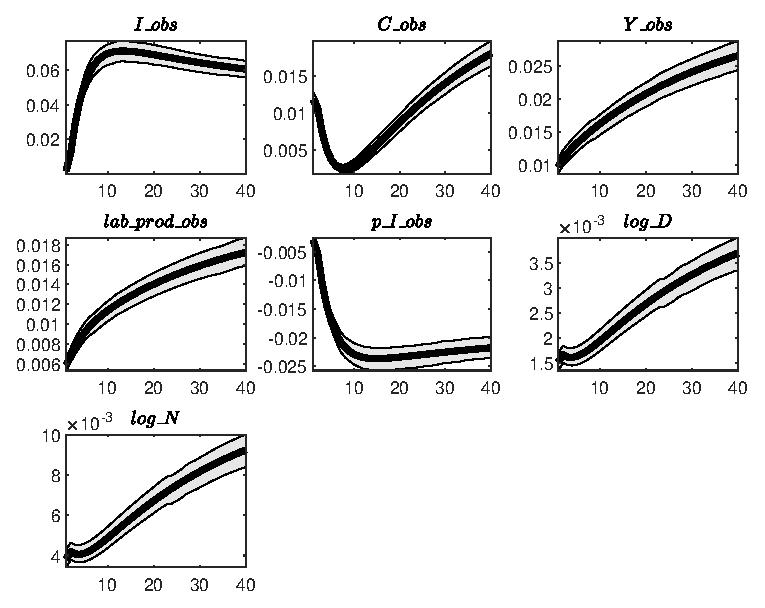
\includegraphics[width=0.80\textwidth]{BRS/Output/BRS_Bayesian_IRF_e_Z_1}
\caption{Bayesian IRF: Orthogonalized shock to ${e_Z}$.}
\label{Fig:BayesianIRF:e_Z:1}
\end{figure}
 
\begin{figure}[H]
\centering 
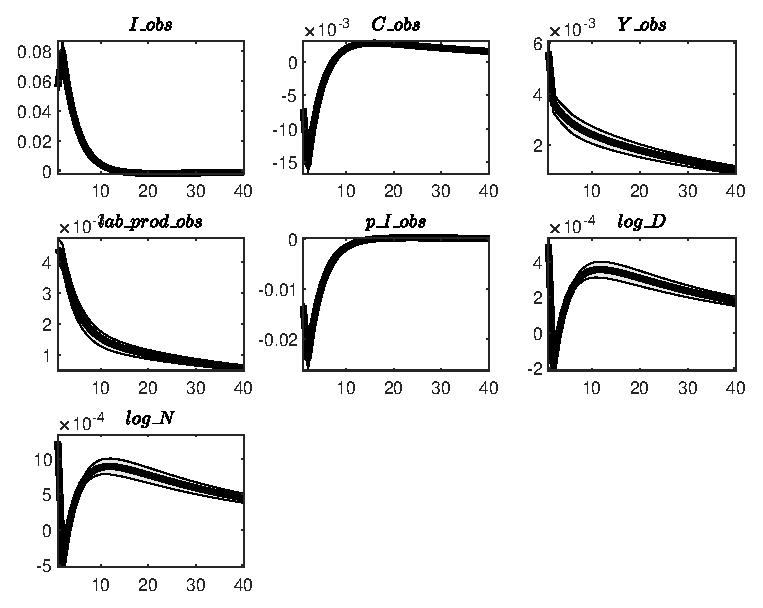
\includegraphics[width=0.80\textwidth]{BRS/Output/BRS_Bayesian_IRF_e_ZI_1}
\caption{Bayesian IRF: Orthogonalized shock to ${e_ZI}$.}
\label{Fig:BayesianIRF:e_ZI:1}
\end{figure}
 
\begin{figure}[H]
\centering 
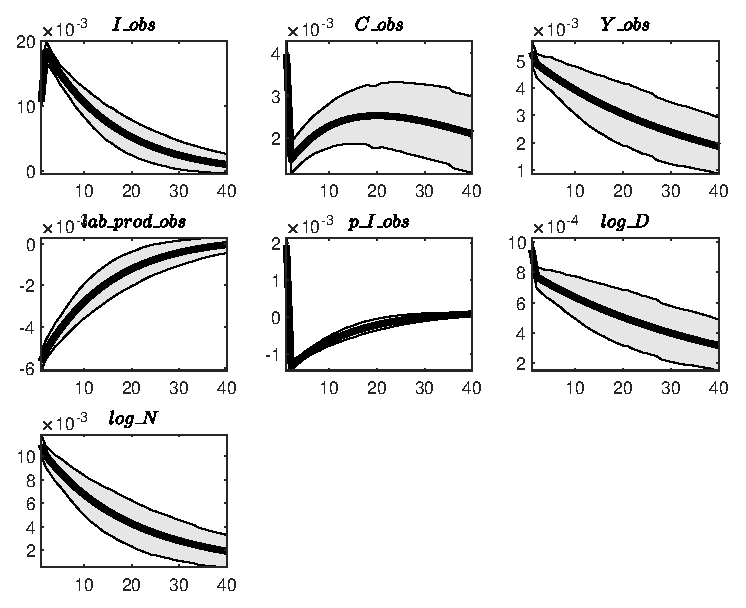
\includegraphics[width=0.80\textwidth]{BRS/Output/BRS_Bayesian_IRF_e_N_1}
\caption{Bayesian IRF: Orthogonalized shock to ${e_N}$.}
\label{Fig:BayesianIRF:e_N:1}
\end{figure}
 
\begin{figure}[H]
\centering 
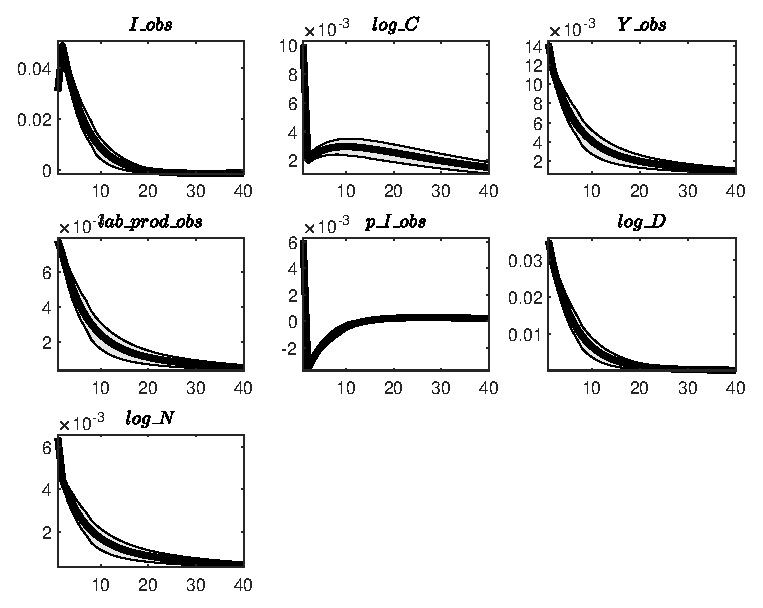
\includegraphics[width=0.80\textwidth]{BRS/Output/BRS_Bayesian_IRF_e_D_1}
\caption{Bayesian IRF: Orthogonalized shock to ${e_D}$.}
\label{Fig:BayesianIRF:e_D:1}
\end{figure}
 
% End of TeX file.
 
% TeX eps-loader file generated by McmcDiagnostics.m (Dynare).
% 21-Jan-2024 18:58:04
 
\begin{figure}[H]
\centering 
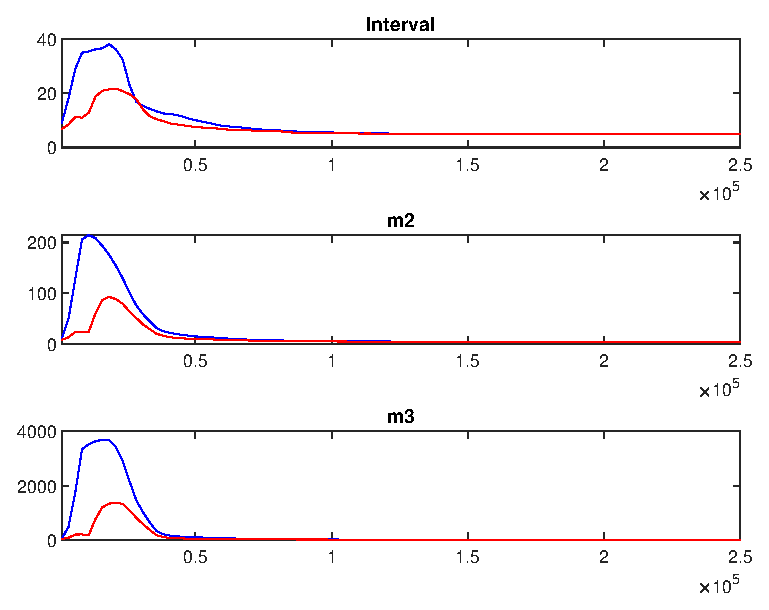
\includegraphics[width=0.8\textwidth]{BRS/Output/BRS_mdiag}
\caption{Multivariate convergence diagnostics for the Metropolis-Hastings.
The first, second and third rows are respectively the criteria based on
the eighty percent interval, the second and third moments. The different 
parameters are aggregated using the posterior kernel.}\label{Fig:MultivariateDiagnostics}
\end{figure}

% End Of TeX file. 
% TeX-table generated by Dynare.
% RESULTS FROM METROPOLIS HASTINGS (parameters)
% 23-Jan-2024 12:12:10 
 
\begin{center}
\begin{longtable}{llcccccc} 
\caption{Results from Metropolis-Hastings (parameters)}
 \label{Table:MHPosterior:1}\\
\toprule 
  & \multicolumn{3}{c}{Prior}  &  \multicolumn{4}{c}{Posterior} \\
  \cmidrule(r{.75em}){2-4} \cmidrule(r{.75em}){5-8}
  & Dist. & Mean  & Stdev. & Mean & Stdev. & HPD inf & HPD sup\\
\midrule \endfirsthead 
\caption{(continued)}\\\toprule 
  & \multicolumn{3}{c}{Prior}  &  \multicolumn{4}{c}{Posterior} \\
  \cmidrule(r{.75em}){2-4} \cmidrule(r{.75em}){5-8}
  & Dist. & Mean  & Stdev. & Mean & Stdev. & HPD inf & HPD sup\\
\midrule \endhead 
\bottomrule \multicolumn{8}{r}{(Continued on next page)} \endfoot 
\bottomrule \endlastfoot 
${\rho_Z}$ & beta &   0.600 & 0.2000 &   0.999& 0.0005 &  0.9985 &  0.9999 \\ 
${\rho_ZI}$ & beta &   0.600 & 0.2000 &   0.733& 0.0124 &  0.7125 &  0.7541 \\ 
 
% TeX-table generated by Dynare.
% RESULTS FROM METROPOLIS HASTINGS (standard deviation of structural shocks)
% 23-Jan-2024 16:35:31 
 
\begin{center}
\begin{longtable}{llcccccc} 
\caption{Results from Metropolis-Hastings (standard deviation of structural shocks)}
 \label{Table:MHPosterior:2}\\
\toprule 
  & \multicolumn{3}{c}{Prior}  &  \multicolumn{4}{c}{Posterior} \\
  \cmidrule(r{.75em}){2-4} \cmidrule(r{.75em}){5-8}
  & Dist. & Mean  & Stdev. & Mean & Stdev. & HPD inf & HPD sup\\
\midrule \endfirsthead 
\caption{(continued)}\\\toprule 
  & \multicolumn{3}{c}{Prior}  &  \multicolumn{4}{c}{Posterior} \\
  \cmidrule(r{.75em}){2-4} \cmidrule(r{.75em}){5-8}
  & Dist. & Mean  & Stdev. & Mean & Stdev. & HPD inf & HPD sup\\
\midrule \endhead 
\bottomrule \multicolumn{8}{r}{(Continued on next page)} \endfoot 
\bottomrule \endlastfoot 
${e_ZI}$ & invg &   0.010 & 0.1000 &   0.025& 0.0013 &  0.0224 &  0.0266 \\ 
${e_Z}$ & invg &   0.010 & 0.1000 &   0.008& 0.0005 &  0.0067 &  0.0083 \\ 
${e_N}$ & invg &   0.010 & 0.1000 &   0.021& 0.0011 &  0.0187 &  0.0221 \\ 
${e_D}$ & invg &   0.010 & 0.1000 &   0.195& 0.0040 &  0.1899 &  0.2000 \\ 
\end{longtable}
 \end{center}
% End of TeX file.
 
% TeX-table generated by dynare_estimation (Dynare).
% RESULTS FROM POSTERIOR MAXIMIZATION (parameters)
% 23-Jan-2024 16:35:02 
 
\begin{center}
\begin{longtable}{llcccc} 
\caption{Results from posterior maximization (parameters)}\\
 \label{Table:Posterior:1}\\
\toprule 
  & \multicolumn{3}{c}{Prior}  &  \multicolumn{2}{c}{Posterior} \\
  \cmidrule(r{.75em}){2-4} \cmidrule(r{.75em}){5-6}
  & Dist. & Mean  & Stdev & Mode & Stdev \\ 
\midrule \endfirsthead 
\caption{(continued)}\\
 \bottomrule 
  & \multicolumn{3}{c}{Prior}  &  \multicolumn{2}{c}{Posterior} \\
  \cmidrule(r{.75em}){2-4} \cmidrule(r{.75em}){5-6}
  & Dist. & Mean  & Stdev & Mode & Stdev \\ 
\midrule \endhead 
\bottomrule \multicolumn{6}{r}{(Continued on next page)}\endfoot 
\bottomrule\endlastfoot 
${\rho_Z}$ & beta &   0.600 & 0.2000 &   0.8997 &  0.0313 \\ 
${\rho_ZI}$ & beta &   0.600 & 0.2000 &   0.9729 &  0.0138 \\ 
${\rho_N}$ & beta &   0.600 & 0.2000 &   0.9458 &  0.0174 \\ 
${\rho_D}$ & beta &   0.600 & 0.2000 &   0.7819 &  0.0399 \\ 
\end{longtable}
 \end{center}
% End of TeX file.
 
% TeX-table generated by dynare_estimation (Dynare).
% RESULTS FROM POSTERIOR MAXIMIZATION (standard deviation of structural shocks)
% 19-Jan-2024 15:47:58 
 
\begin{center}
\begin{longtable}{llcccc} 
\caption{Results from posterior maximization (standard deviation of structural shocks)}\\
 \label{Table:Posterior:2}\\
\toprule 
  & \multicolumn{3}{c}{Prior}  &  \multicolumn{2}{c}{Posterior} \\
  \cmidrule(r{.75em}){2-4} \cmidrule(r{.75em}){5-6}
  & Dist. & Mean  & Stdev & Mode & Stdev \\ 
\midrule \endfirsthead 
\caption{(continued)}\\
 \bottomrule 
  & \multicolumn{3}{c}{Prior}  &  \multicolumn{2}{c}{Posterior} \\
  \cmidrule(r{.75em}){2-4} \cmidrule(r{.75em}){5-6}
  & Dist. & Mean  & Stdev & Mode & Stdev \\ 
\midrule \endhead 
\bottomrule \multicolumn{6}{r}{(Continued on next page)}\endfoot 
\bottomrule\endlastfoot 
${e_ZI}$ & invg &   0.010 & 0.1000 &   0.0306 &  0.0019 \\ 
${e_Z}$ & invg &   0.010 & 0.1000 &   0.0062 &  0.0006 \\ 
${e_N}$ & invg &   0.010 & 0.1000 &   0.0203 &  0.0010 \\ 
${e_D}$ & invg &   0.010 & 0.1000 &   0.1978 &  0.0102 \\ 
\end{longtable}
 \end{center}
% End of TeX file.
 
% TeX eps-loader file generated by PlotPosteriorDistributions.m (Dynare).
% 19-Jan-2024 16:02:07
 
\begin{figure}[H]
\centering
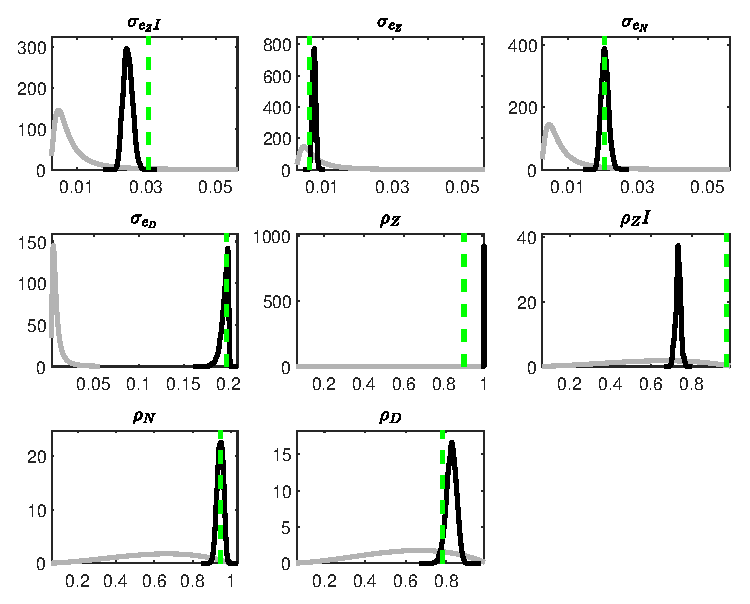
\includegraphics[width=0.80\textwidth]{BRS/Output/BRS_PriorsAndPosteriors1}
\caption{Priors and posteriors.}\label{Fig:PriorsAndPosteriors:1}
\end{figure}
 
% End of TeX file.
 
% TeX eps-loader file generated by McmcDiagnostics.m (Dynare).
% 23-Jan-2024 16:35:14
 
\begin{figure}[H]
\centering 
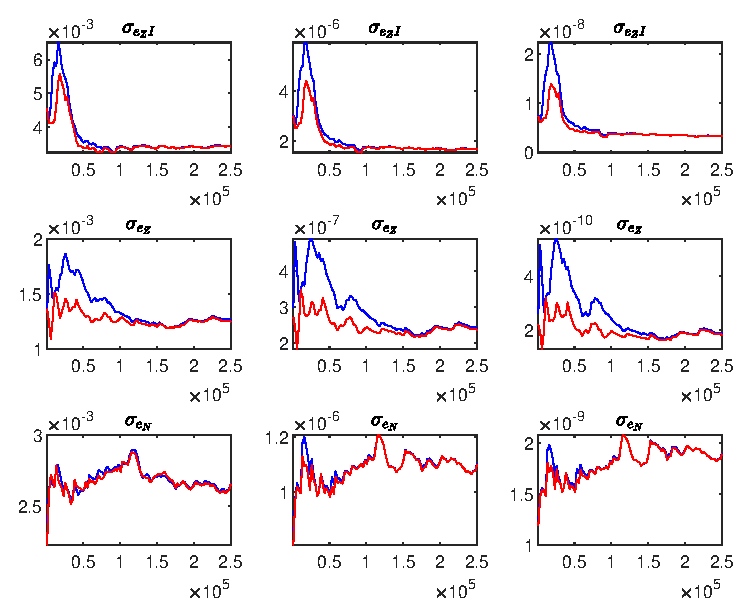
\includegraphics[width=0.80\textwidth]{BRS/Output/BRS_udiag1}
\caption{Univariate convergence diagnostics for the Metropolis-Hastings.
The first, second and third columns are respectively the criteria based on
the eighty percent interval, the second and third moments.}\label{Fig:UnivariateDiagnostics:1}
\end{figure}

\begin{figure}[H]
\centering 
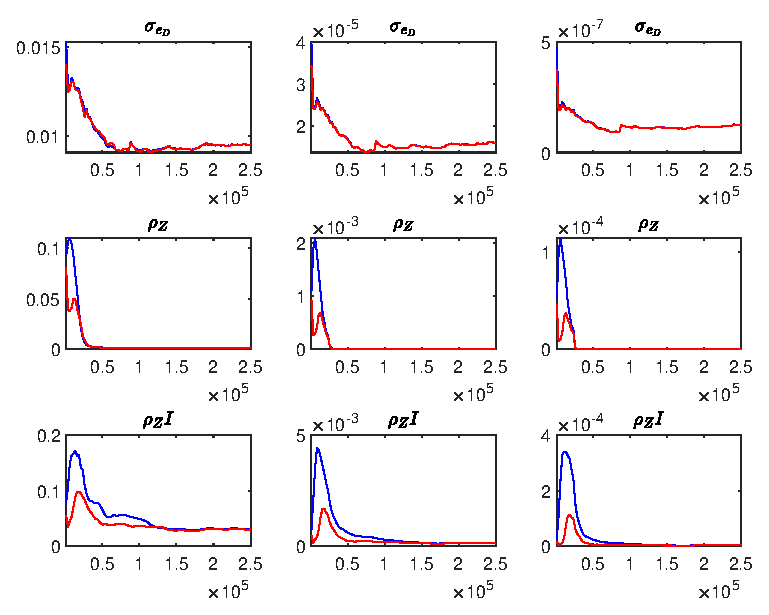
\includegraphics[width=0.80\textwidth]{BRS/Output/BRS_udiag2}
\caption{Univariate convergence diagnostics for the Metropolis-Hastings.
The first, second and third columns are respectively the criteria based on
the eighty percent interval, the second and third moments.}\label{Fig:UnivariateDiagnostics:2}
\end{figure}

\begin{figure}[H]
\centering 
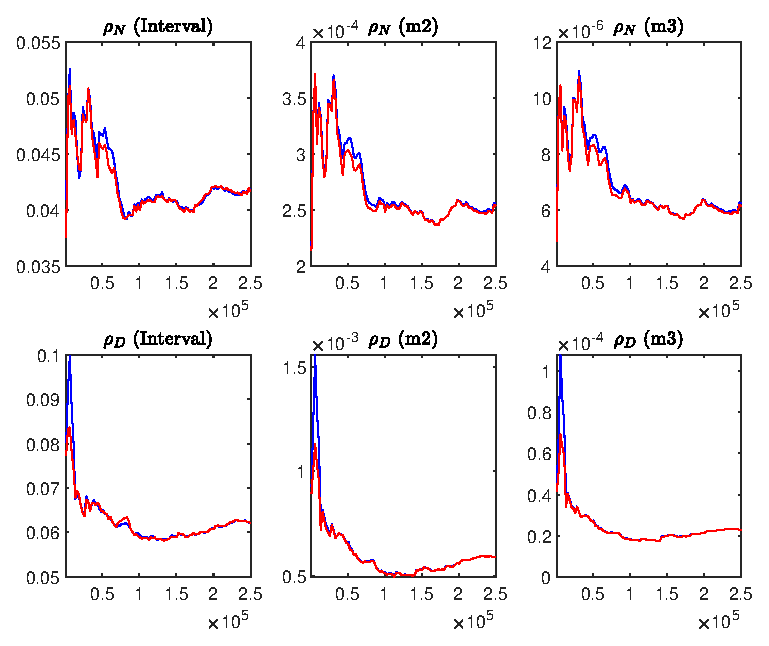
\includegraphics[width=0.80\textwidth]{BRS/Output/BRS_udiag3}
\caption{Univariate convergence diagnostics for the Metropolis-Hastings.
The first, second and third columns are respectively the criteria based on
the eighty percent interval, the second and third moments.}\label{Fig:UnivariateDiagnostics:3}
\end{figure}

 
% TeX eps-loader file generated by mode_check.m (Dynare).
% 19-Jan-2024 15:47:56
 
\begin{figure}[H]
\centering 
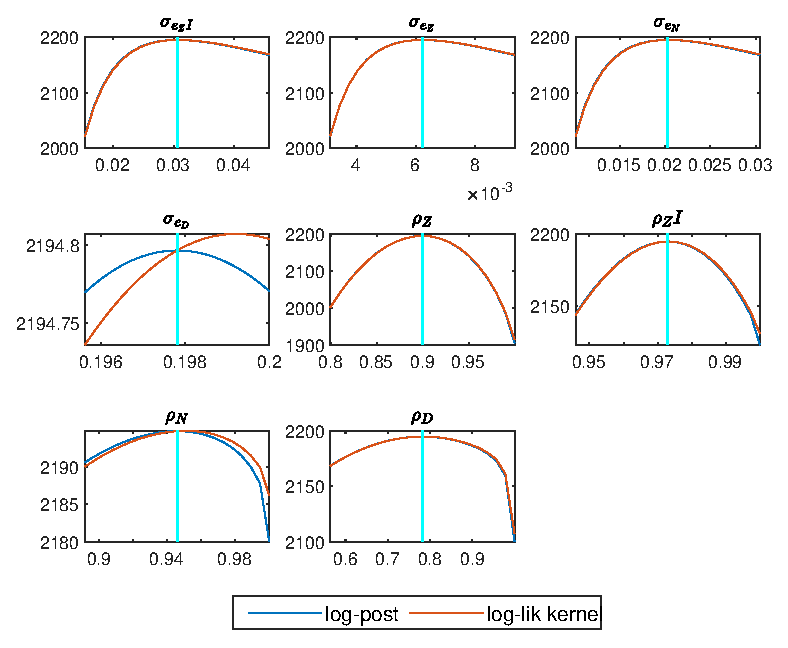
\includegraphics[width=0.80\textwidth]{BRS/graphs/BRS_CheckPlots1}
\caption{Check plots.}\label{Fig:CheckPlots:1}
\end{figure}
 
 
% TeX eps-loader file generated by dynare_estimation_1.m (Dynare).
% 19-Jan-2024 16:02:38
 
\begin{figure}[H]
\centering 
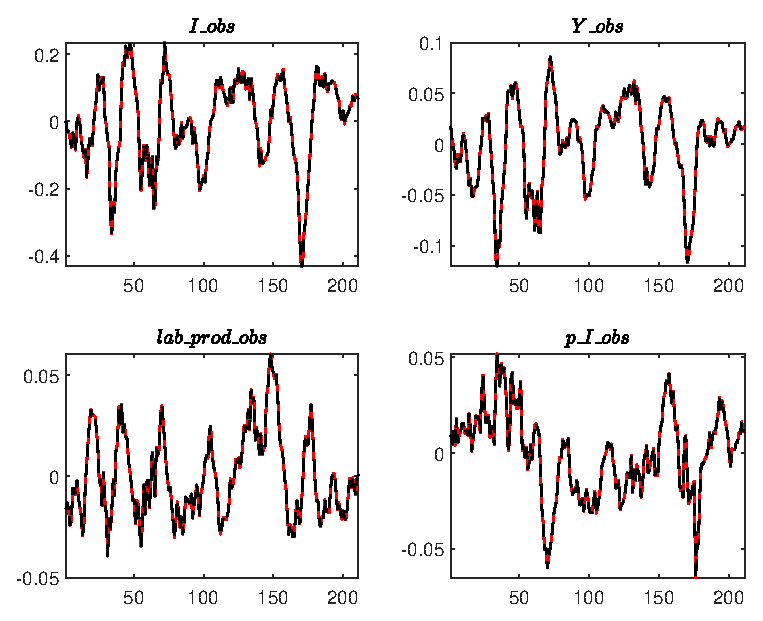
\includegraphics[width=0.80\textwidth]{BRS/graphs/BRS_HistoricalAndSmoothedVariables1}
\caption{Historical and smoothed variables.}\label{Fig:HistoricalAndSmoothedVariables:1}
\end{figure}


% End of TeX file.
 
% TeX eps-loader file generated by plot_priors.m (Dynare).
% 23-Jan-2024 12:11:42
 
\begin{figure}[H]
\centering
\includegraphics[width=0.80\textwidth]{BRS/graphs/BRS_Priors1}
\caption{Priors.}\label{Fig:Priors:1}
\end{figure}
 
% End of TeX file.
 
% TeX eps-loader file generated by dynare_estimation_1.m (Dynare).
% 23-Jan-2024 16:36:11
 
\begin{figure}[H]
\centering 
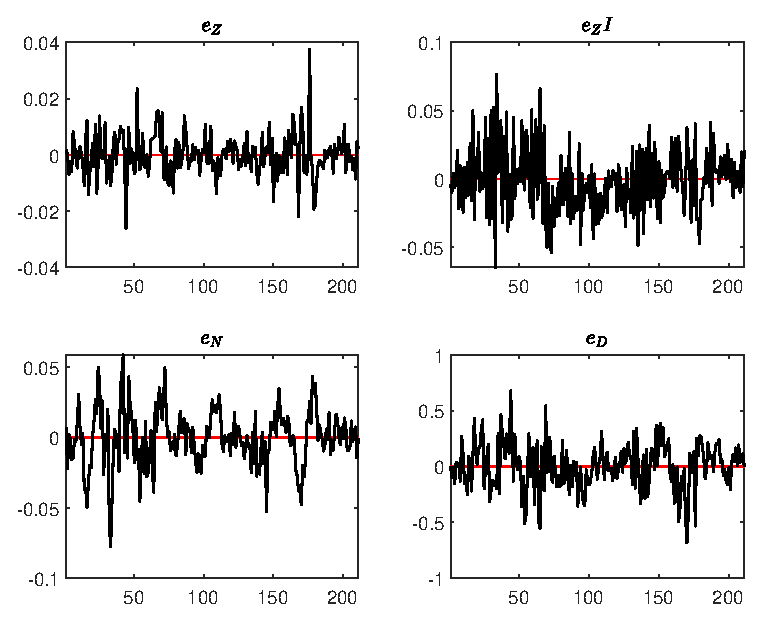
\includegraphics[width=0.80\textwidth]{BRS/graphs/BRS_SmoothedShocks1}
\caption{Smoothed shocks.}\label{Fig:SmoothedShocks:1}
\end{figure}


% End of TeX file.
 
\include{BRS/graphs/BRS_TracePlot_Posterior_blck_1} 
\include{BRS/graphs/BRS_TracePlot_SE_e_D_blck_1} 
\include{BRS/graphs/BRS_TracePlot_SE_e_N_blck_1} 
\include{BRS/graphs/BRS_TracePlot_SE_e_ZI_blck_1} 
\include{BRS/graphs/BRS_TracePlot_SE_e_Z_blck_1} 
\include{BRS/graphs/BRS_TracePlot_rho_D_blck_1} 
\include{BRS/graphs/BRS_TracePlot_rho_N_blck_1} 
\include{BRS/graphs/BRS_TracePlot_rho_ZI_blck_1} 
\include{BRS/graphs/BRS_TracePlot_rho_Z_blck_1} 
\end{document} 
